\section{The cube structure}
%In this section the different classes of the \rubik{} and their interaction with each other will be determined.
In this implementation we used a more object orientated approach to the problem.
The \rubik{} is divided into its sub structures which consist of six faces each with nine shared \cubicle{}s each containing a \cubie{}. The \cubie{}s either consist of one, two or three facelets. On figure \ref{fig:cubeClassDiagram} the cube class diagram is shown and a detailed description of the classes will explained in the following subsections.
%The cube consist of the 6 faces each with 9 shared \cpiece{}. 

\begin{figure}[htbp]
	\centering
		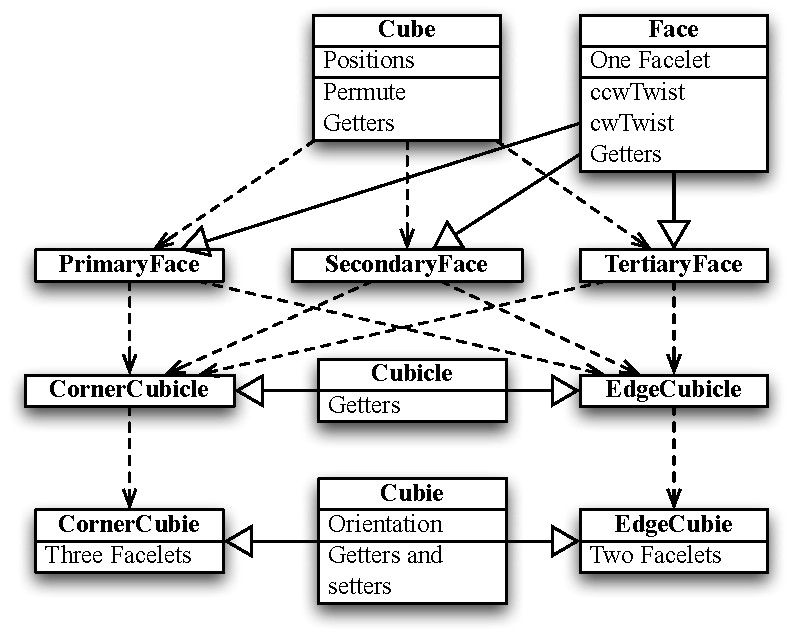
\includegraphics{input/pics/cubeClassDiagram.pdf}
	\caption{Class diagram of the cube with attribute and properties}
	\label{fig:cubeClassDiagram}
\end{figure}


There are three types of \cpiece{}s and \cubicle{}s: corners, edges, and centers. 

\subsection{The Cube}
The cube class creates the 20 \cubicle{}s in which the \cpiece{}s can be positioned. Furthermore the cube class creates the \face{}s and \cubie{}s. Eventhough the cube class initialize all objects this is not drawn on the class diagram (figure \ref{fig:cubeClassDiagram}) because they are not used this way. The cube class also gives each \cpiece{} its \facelet{}s. The \cubicle{}s are then put into a \face{} by its constructor. The cube class creates six \face{}s -- two primary, two secondary and two tertiary faces. Each type of \face{}s are placed opposite to each other. e.g. the up and down faces are both primary. The cube has a static method, \vr{permute}, it has two arguments, a cube and a sequence of \twist{}. The \twist{}s are applied to the cube.

\subsection{The Face}
A face consists of nine \cubicle{}s which act as placeholders for the \cpiece{}s. The center \cpiece{}s will never move and therefore there is no reason to define a \cubicle{} and a \cpiece{} for those. Instead the center piece of a face is granted a colored \facelet{}, which defines the color of the face in the completed state of the \rubik{}.
The \face{} class constructor takes eight cubicles (four corners and four edges) and position them in a clockwise order. In addition the \face{} class implements two methods which twist the face clockwise or counterclockwise -- namely \textit{cwTwist} and \textit{ccwTwist} respectively.

There are three different types of \face{}s; primary \face{}s, secondary \face{}s, and tertiary \face{}s.
Each type has its own subclass, which inherits from the \face{} superclass.
The reason for the different classes is that there is a difference in how the orientation of the \cubie{}s changes depending on what type of \face{} being \twist{}ed.
%Orientation of \cubie{}s will be covered in ref\{orientation\}.

\subsection{The Cubicle}
%Måske noget om cubicle class, hvis der bliver lavet noget.
The \cubicle{} class is a superclass and there are two subclasses to this class corner- and edge \cubicle{}.
The corner and edge \cubicle{} classes each has one instance variable, namely the \cubie{} they hold. The \cpiece{} is set by the constructor of the \cubicle{} class.

\subsection{The Cubie}
The \cpiece{} class sets the orientation correctly by default, and it implements methods that return the orientation and \facelet{}s of the \cpiece{}. The corner and edge \cpiece{} classes implements two different methods which return the orientation of the \cpiece{}. The \cubie{} class is a superclass and there are two subclasses to this corner- and edge \cubie{}. The corner \cubie{} contains three facelets, where edge \cubie{} only contains two facelets.

\subsection{The Facelet}
%%The \facelet{} class is an enumeration that contains the colors of the \facelet{}s, it implements a \textit{toColor} method which define the color of each \facelet{}.
The \facelet{}s are defined in an enumeration which contains the colors of the \facelet{}s, it implements a \textit{toColor} method which define the actual color of each \facelet{}.